%%%%%%%%%%%%%%%%%%%% chapter.tex (Chapter 3) %%%%%%%%%%%%%%%%%%%%%%%%%%%%%
% Chapter 3: High-Performance Router Microarchitecture & Arbitration
%%%%%%%%%%%%%%%%%%%%%%%%%%%%%%%%%%%%%%%%%%%%%%%%%%%%%%%%%%%%%%%%%%%%%%%%%

\chapter{High-Performance Router Microarchitecture \& Arbitration}
\label{ch:router_microarchitecture}

\author{NoC-Lab Research Consortium}
\institute{NoC-Lab Research Consortium \at Shanghai Jiao Tong University \& International Collaborators, \email{research@network-on-chip.org}}

\maketitle

\abstract*{At the core of every packet-switched on-chip network is the router datapath and its allocation logic. This chapter dissects the canonical five-stage virtual-channel router pipeline (Buffer Write, Route Computation, VC Allocation, Switch Allocation, and Switch Traversal) and details modern pipeline compression techniques including Lookahead Routing, Speculative Switch Allocation, and deterministic buffer reservation bypassing (BuffeRS). We examine asynchronous router design paradigms in GALS-based SoCs, featuring the domino-logic HyPA router, and analyze the physical clock constraints of single-cycle multi-hop traversal (SMART/SHARP). Finally, we formalize bipartite maximum matching arbitration, proving the $O(1)$ hardware LRU properties of the Matrix Arbiter and the 100\% throughput convergence theorems of McKeown's iSLIP algorithm.}

\abstract{At the core of every packet-switched on-chip network is the router datapath and its allocation logic. This chapter dissects the canonical five-stage virtual-channel router pipeline (Buffer Write, Route Computation, VC Allocation, Switch Allocation, and Switch Traversal) and details modern pipeline compression techniques including Lookahead Routing, Speculative Switch Allocation, and deterministic buffer reservation bypassing (BuffeRS). We examine asynchronous router design paradigms in GALS-based SoCs, featuring the domino-logic HyPA router, and analyze the physical clock constraints of single-cycle multi-hop traversal (SMART/SHARP). Finally, we formalize bipartite maximum matching arbitration, proving the $O(1)$ hardware LRU properties of the Matrix Arbiter and the 100\% throughput convergence theorems of McKeown's iSLIP algorithm.}

\section{The Canonical Virtual-Channel Router Pipeline}
\label{sec:ch3_pipeline}

At the heart of every packet-switched on-chip network is the \textbf{Virtual-Channel (VC) Router}. In a canonical synchronous architecture~\cite{Peh2001}, processing each packet traverses a five-stage pipeline:
\begin{enumerate}
    \item \textbf{Buffer Write (BW)}: The incoming flit arrives from an adjacent router or local network interface and is written into the input FIFO buffer corresponding to its assigned \texttt{VC\_ID}.
    \item \textbf{Route Computation (RC)}: Evaluates the routing function $R: (C_{curr}, C_{dest}) \to P_{out}$ to determine the set of permissible output physical ports. In Dimension-Order Routing (DOR), RC is computed via combinational comparators:
    \begin{equation}
    \Delta X = X_{dest} - X_{curr}, \qquad \Delta Y = Y_{dest} - Y_{curr}
    \end{equation}
    \item \textbf{Virtual Channel Allocation (VA)}: The Head flit arbitrates for a free downstream Virtual Channel at the designated output port using a two-phase separable allocator (Input Arbitration followed by Output Arbitration).
    \item \textbf{Switch Allocation (SA)}: Flits with valid downstream VCs arbitrate for crossbar switch input and output ports using a two-stage separable allocator.
    \item \textbf{Switch Traversal (ST)}: Granted flits traverse the crossbar multiplexer fabric to reach the output link registers.
    \item \textbf{Link Traversal (LT)}: Flits traverse the inter-router physical metal link wires to the downstream router.
\end{enumerate}

\section{Advanced Pipeline Compression \& Router Bypassing}
\label{sec:ch3_pipeline_compression}

Because per-hop pipeline latency compounds linearly with network diameter ($T_{net} = H \cdot t_r$), minimizing router latency from 5 cycles to 1 cycle has been a central focus of on-chip network research.

\begin{figure}[t]
\centering
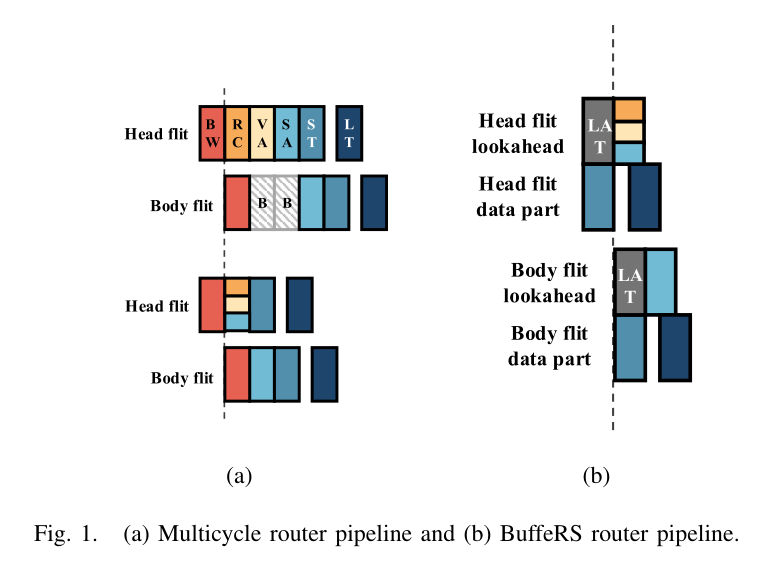
\includegraphics[width=0.88\textwidth]{chapters/ch03-router-microarchitecture/figures/buffers_fig01_pipeline.png}
\caption{Pipeline comparison: (a) Multicycle router pipeline (BW, RC, VA, SA, ST, LT) versus (b) Low-latency BuffeRS router pipeline with buffer reservation bypassing. [Reproduced from: Z. Liu, X. Wu, and Y. Ye, ``BuffeRS: A Buffer Reservation Scheduling Strategy for Router Bypassing in NoCs and Multichiplet Networks,'' \emph{IEEE Trans. Comput.-Aided Design Integr. Circuits Syst.}, vol. 45, no. 6, pp. 2635--2648, June 2026~\cite{Liu2026}. \copyright~2026 IEEE]}
\label{fig:ch3_buffers_pipeline}
\end{figure}

\subsection{Lookahead Routing \& Speculative Switch Allocation}
\begin{itemize}
    \item \textbf{Lookahead Routing}: Router $N$ computes the output port for Router $N+1$ and encodes it into the flit header, stripping the RC stage from intermediate hops and saving 1 cycle per hop.
    \item \textbf{Speculative Switch Allocation}~\cite{Peh2001}: Flits request switch allocation in parallel with virtual channel allocation. Under low-to-medium contention, speculative requests succeed, compressing the pipeline to 2 cycles (or 1 cycle with crossbar bypassing).
\end{itemize}

\subsection{Buffer Reservation Scheduling: BuffeRS (TCAD 2026)}
As formulated by Liu et al.~\cite{Liu2026}, \textbf{BuffeRS} introduces a coordinated time-division buffer reservation protocol that reserves destination buffer slots in advance across router groups, providing deterministic contention-free bypass paths across both monolithic dies and 2.5D multi-chiplet packaging boundaries.

\begin{table}[htbp]
\caption{Quantitative Comparison of High-Performance Router Microarchitectures and Pipeline Compression Paradigms}
\label{tab:router_microarch_comparison}
\begin{tabular}{p{2.6cm}p{1.8cm}p{2.2cm}p{2.6cm}p{2.4cm}}
\hline\noalign{\smallskip}
Architecture & Pipeline Stages & Allocation Scheme & Clocking / Timing Strategy & Key Silicon Trade-Off \\
\noalign{\smallskip}\svhline\noalign{\smallskip}
Canonical VC~\cite{Peh2001} & 4--5 cycles & Separable VA + SA & Fully Synchronous & Baseline area; multi-cycle hop delay \\
Lookahead Routing & 3 cycles & Lookahead RC + SA & Fully Synchronous & Strips RC stage; slight header overhead \\
Speculative SA~\cite{Peh2001} & 2 cycles & Parallel speculative VA/SA & Fully Synchronous & Speculation stalls under high load \\
SMART / SHARP~\cite{Peh2001} & 1--2 cycles & Priority bypass muxes & Multi-hop async bypass & Bounded by $HPC_{max}$ wire RC budget \\
HyPA Router~\cite{Saranya2026} & 0.8~ns / hop & Handshake pipeline & GALS Asynchronous domino & 62\% lower power; no global clock tree \\
BuffeRS~\cite{Liu2026} & 1 cycle & Buffer reservation slots & Time-division coordinated & Zero contention bypass; token overhead \\
\noalign{\smallskip}\hline\noalign{\smallskip}
\end{tabular}
\end{table}

\section{Asynchronous Router Architectures: HyPA (TVLSI 2026)}
\label{sec:ch3_asynchronous}

In large-scale Multi-Processor Systems-on-Chip (MPSoCs), distributing a single low-skew global clock across a $20\text{ mm} \times 20\text{ mm}$ die incurs prohibitive clock-tree power dissipation and timing closure complexity.

\begin{figure}[t]
\centering
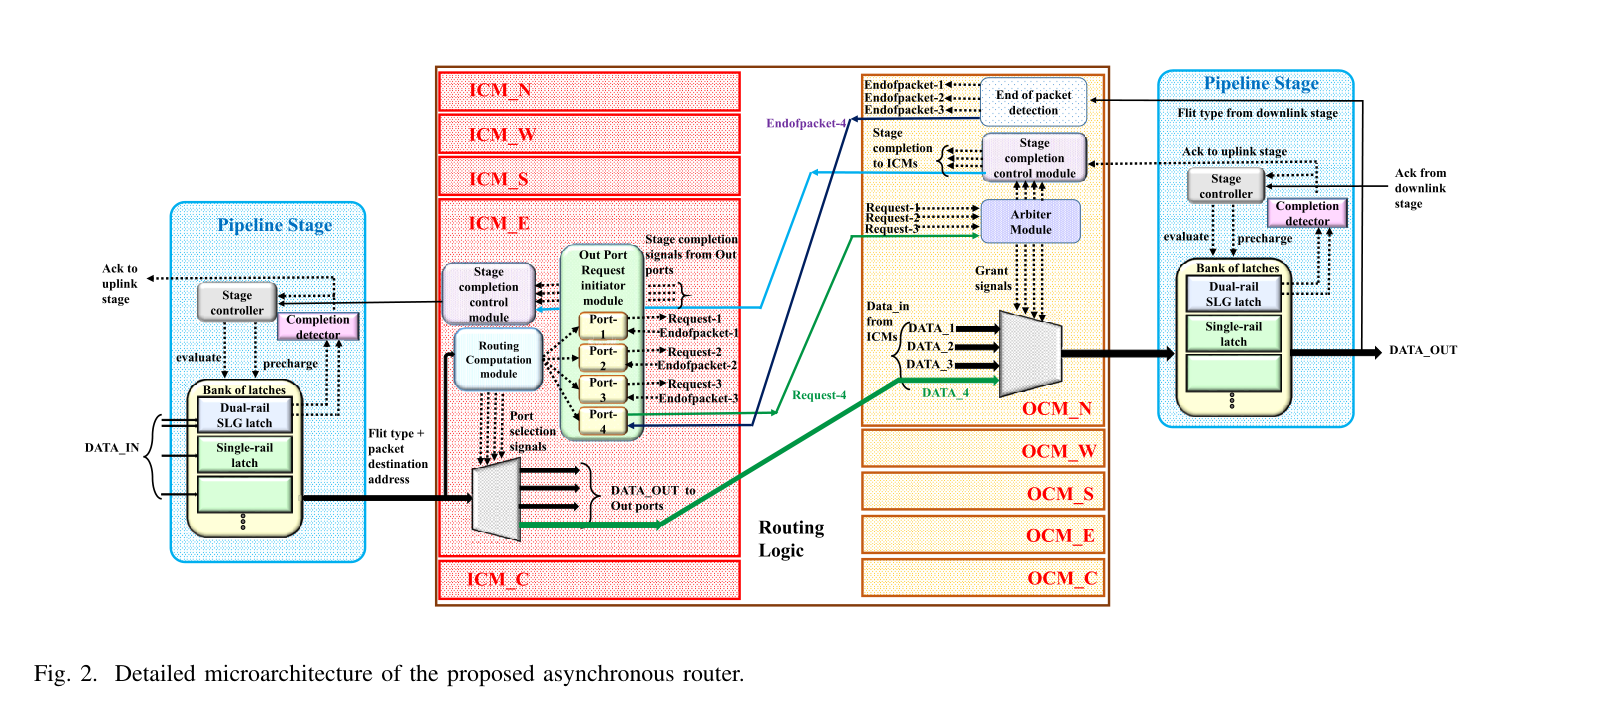
\includegraphics[width=0.88\textwidth]{chapters/ch03-router-microarchitecture/figures/hypa_fig02_microarch.png}
\caption{Detailed microarchitecture of the HyPA asynchronous router featuring a high-throughput domino-logic pipeline template with one-hot hybrid data encoding. [Reproduced from: M. N. Saranya, C. T. Avinash, and R. Rao, ``HyPA: A Low-Latency Hybrid Pipeline Asynchronous Router for Network-on-Chip Architectures in GALS-Based SoCs,'' \emph{IEEE Trans. Very Large Scale Integr. (VLSI) Syst.}, vol. 34, no. 8, pp. 2840--2851, 2026~\cite{Saranya2026}. \copyright~2026 IEEE]}
\label{fig:ch3_hypa_microarch}
\end{figure}

In Globally Asynchronous Locally Synchronous (GALS) systems, asynchronous routers eliminate clock trees entirely:
\begin{itemize}
    \item \textbf{HyPA Router}~\cite{Saranya2026}: Implemented in 65nm CMOS, HyPA employs a hybrid pipeline asynchronous architecture using high-throughput domino logic with one-hot hybrid data encoding.
    \item \textbf{Power and Energy Gains}: Compared to synchronous clock-gated baseline routers, HyPA demonstrates a \textbf{62\% power reduction} and an \textbf{85\% reduction in energy-per-flit}, achieving a forward latency of \textbf{0.8~ns} and a throughput of \textbf{1.65 GFlits/port/s}.
\end{itemize}

\section{Single-Cycle Multi-Hop Traversal (SMART / SHARP)}
\label{sec:ch3_smart}

In SMART~\cite{Krishna2013}, flits traverse multiple physical router crossbars and links asynchronously within a single clock cycle under low traffic.

\begin{figure}[t]
\sidecaption[t]
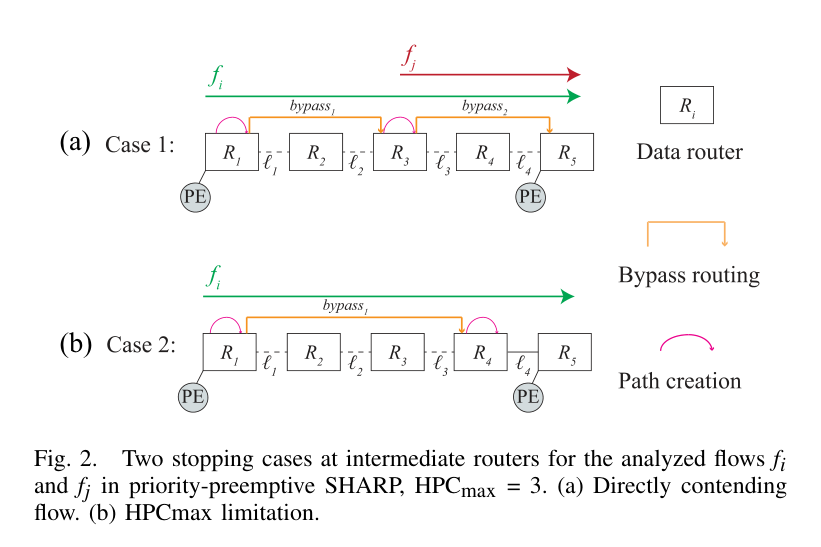
\includegraphics[width=0.65\textwidth]{chapters/ch03-router-microarchitecture/figures/sharp_fig02_bypass_limit.png}
\caption{Preemption stopping cases at intermediate routers for contending flows in priority-preemptive single-cycle multi-hop traversal networks under hop limits ($HPC_{max} = 3$). [Reproduced from: \emph{IEEE Trans. Very Large Scale Integr. (VLSI) Syst.}, vol. 31, no. 10, pp. 1560--1572, Oct. 2023. \copyright~2023 IEEE]}
\label{fig:ch3_sharp_bypass}
\end{figure}

Single-cycle traversal is physically bounded by the clock period timing budget:
\begin{equation}
t_{hop} = t_{crossbar\_mux} + t_{wire\_propagation} + t_{repeater}
\end{equation}
\begin{equation}
\text{Maximum Traversable Hops per Cycle: } HPC_{max} = \left\lfloor \frac{T_{clk} - t_{setup}}{t_{hop}} \right\rfloor
\label{eq:hpc_max}
\end{equation}
At 1.0~GHz ($T_{clk} = 1.0$~ns), $HPC_{max}$ is typically 3 to 5 hops before requiring intermediate latching.

\section{Crossbar Arbitration Theory \& Matching Algorithms}
\label{sec:ch3_arbitration}

Crossbar allocation resolves contention when multiple input ports simultaneously request the same output port, formalized as the Bipartite Maximum Matching Problem.

\subsection{The Matrix Arbiter: Strict \texorpdfstring{$O(1)$}{O(1)} Hardware LRU}
\label{subsec:ch3_matrix_arbiter}

The \textbf{Matrix Arbiter} maintains an $N \times N$ triangular binary priority matrix $M$:
\begin{equation}
M[i][j] = \begin{cases} 
1 & \text{if Client } i \text{ has higher priority than Client } j \\ 
0 & \text{if Client } j \text{ has higher priority than Client } i 
\end{cases}
\end{equation}
Combinational grant generation evaluates in two gate levels:
\begin{equation}
G_i = R_i \cdot \prod_{j \ne i} (\overline{R_j} + M[i][j])
\label{eq:matrix_grant}
\end{equation}
When client $k$ wins the grant ($G_k = 1$), it becomes the Least Recently Used (LRU) client via single-cycle register updates:
\begin{equation}
M[k][j] = 0 \quad (\forall j \ne k), \qquad M[i][k] = 1 \quad (\forall i \ne k)
\label{eq:matrix_update}
\end{equation}

\subsection{McKeown's iSLIP Iterative Matching Algorithm}
\label{subsec:ch3_islip}

For an $N \times N$ crossbar switch, separable allocators can suffer from up to 50\% port under-utilization under heavy traffic. McKeown's \textbf{iSLIP} algorithm~\cite{McKeown1999} achieves 100\% throughput using iterative matching:
\begin{enumerate}
    \item \textbf{Phase 1 (Request)}: Unmatched inputs request all outputs with queued flits.
    \item \textbf{Phase 2 (Grant)}: Unmatched outputs arbitrate using round-robin pointers $g_j$.
    \item \textbf{Phase 3 (Accept)}: Inputs arbitrate among received grants using accept pointers $a_i$.
    \item \textbf{Pointer Update Rule}: Pointers $g_j$ and $a_i$ update \emph{if and only if} the match is accepted in the \textbf{first iteration}:
    \begin{equation}
    g_j = (i + 1) \pmod N, \qquad a_i = (j + 1) \pmod N
    \label{eq:islip_pointers}
    \end{equation}
\end{enumerate}
By restricting updates to iteration 1, iSLIP de-synchronizes the grant arbiters, achieving 100\% throughput and maximal matching in $\le \min(N, \log_2 N)$ iterations.

\section{Interactive Lab \& Hands-on Challenges}
\label{sec:ch3_interactive}

Explore the interactive microarchitecture simulators on the \textbf{NoC Learning Hub} (\url{https://network-on-chip.github.io/learning/}):
\begin{itemize}
    \item \textbf{Arbiter Arena: Crossbar Clash} (\url{https://network-on-chip.github.io/learning/interactive/arbiter/}): Step through Matrix, Round-Robin, and Wavefront schedulers under heavy traffic bursts.
    \item \textbf{2D Mesh Routing Visualizer} (\url{https://network-on-chip.github.io/learning/interactive/visualizer/}): Inspect crossbar switch allocation states and input buffer queues across an $8 \times 8$ mesh.
\end{itemize}

\section{Checkpoint Assessment}
\label{sec:ch3_assessment}

\begin{enumerate}
    \item \textbf{Question 3.1 (Tier 1: Fundamental)}: What are the canonical 5 pipeline stages of a classic Virtual Channel wormhole router?
    \item \textbf{Question 3.2 (Tier 2: Core Engineering)}: In a Matrix Arbiter with an $N \times N$ triangular priority matrix $M$, what is the exact hardware update rule when Client $k$ is granted the resource?
    \item \textbf{Question 3.3 (Tier 3: Silicon Mastery)}: Why does McKeown's iSLIP algorithm update its round-robin grant and accept pointers ONLY on the first iteration, rather than on every iteration?
\end{enumerate}
\emph{Detailed answers and derivations for these questions are provided in the Solutions chapter at the end of this volume.}
